%!TEX root = ../thesis.tex

% \vspace{-10pt}

\section{本章の概要}
% 本章では,\ref{sec:oculus-exp-overview}節で実験の概要を示す.また,\ref{sec:oculus-exp-method}節で実験方法,\ref{sec:oculus-exp-result}節で結果と考察について述べる.

本章では,ロボットと歩行者の相互作用を観察し,提案手法を用いて歩行者の軌道を予測する実験を行った結果について述べる.まず,実験の概要を\ref{sec:oculus-exp-overview}節で説明し,次に実験方法を\ref{sec:oculus-exp-method}節で詳述する.最後に,実験結果とその考察を\ref{sec:oculus-exp-result}節で示す.

\section{実験概要}\label{sec:oculus-exp-overview}
本研究の提案手法の有効性を検証するため,実環境においてロボットと歩行者がどのように相互作用するかを観察し,提案手法を用いて行動を予測する実験を行った.実験には20代の男性4名が参加し,そのうち無作為に選ばれた2名のデータを予測用として利用した.

\section{実験方法}\label{sec:oculus-exp-method}
本実験は,丹野らの研究\cite{si2023-tanno}を参考に実施した.実験は\figref{Fig:oculus-exp-overview}に示す室内環境で行い,\figref{fig:tracking-robot}に示す移動ロボット(ORNE-box2\cite{井口颯人2023屋外自律移動ロボットプラットフォーム-orne})を使用した.実験参加者は,移動ロボットの正面から歩行を開始し,事前に指定された目的地(A/B/C)のいずれかまでロボットを避けながら歩行する.各参加者には,各目的地への歩行を3回ずつ行ってもらった.ロボットの行動が歩行者の将来の軌道にどのように影響を与えるかを観察するため,ロボットは0.3m/sの一定速度で直進した後,以下の3つの挙動のいずれかを事前に知らせることなく無作為に選択して実行する.

\begin{itemize}
  \item 速度を変えず直進
  \item 速度を変えず右に避ける
  \item 速度を変えず左に避ける
\end{itemize}

\figref{fig:tracking}に示すように,参加者とロボットの位置はOculus Riftの専用コントローラを用いて計測する.また,正確なトラッキングを行うため,\figref{Fig:oculus-exp-overview}の斜線部に2基の赤外線センサを\figref{Fig:oculus-sensor}のように配置する.取得データは,ETH\cite{pellegrini2009you-eth},UCY\cite{lerner2007crowds-ucy}データセットのフォーマットに準拠する.

予測の評価手順は,\ref{chap:proposed_method}章で行った予備実験と同様とした.ロボットの行動を考慮した軌道予測手法の有効性を評価するため,ロボットの行動を考慮する場合と考慮しない場合の両方で予測を行い,それぞれの結果を比較する.

\begin{figure}[H]
  \centering
 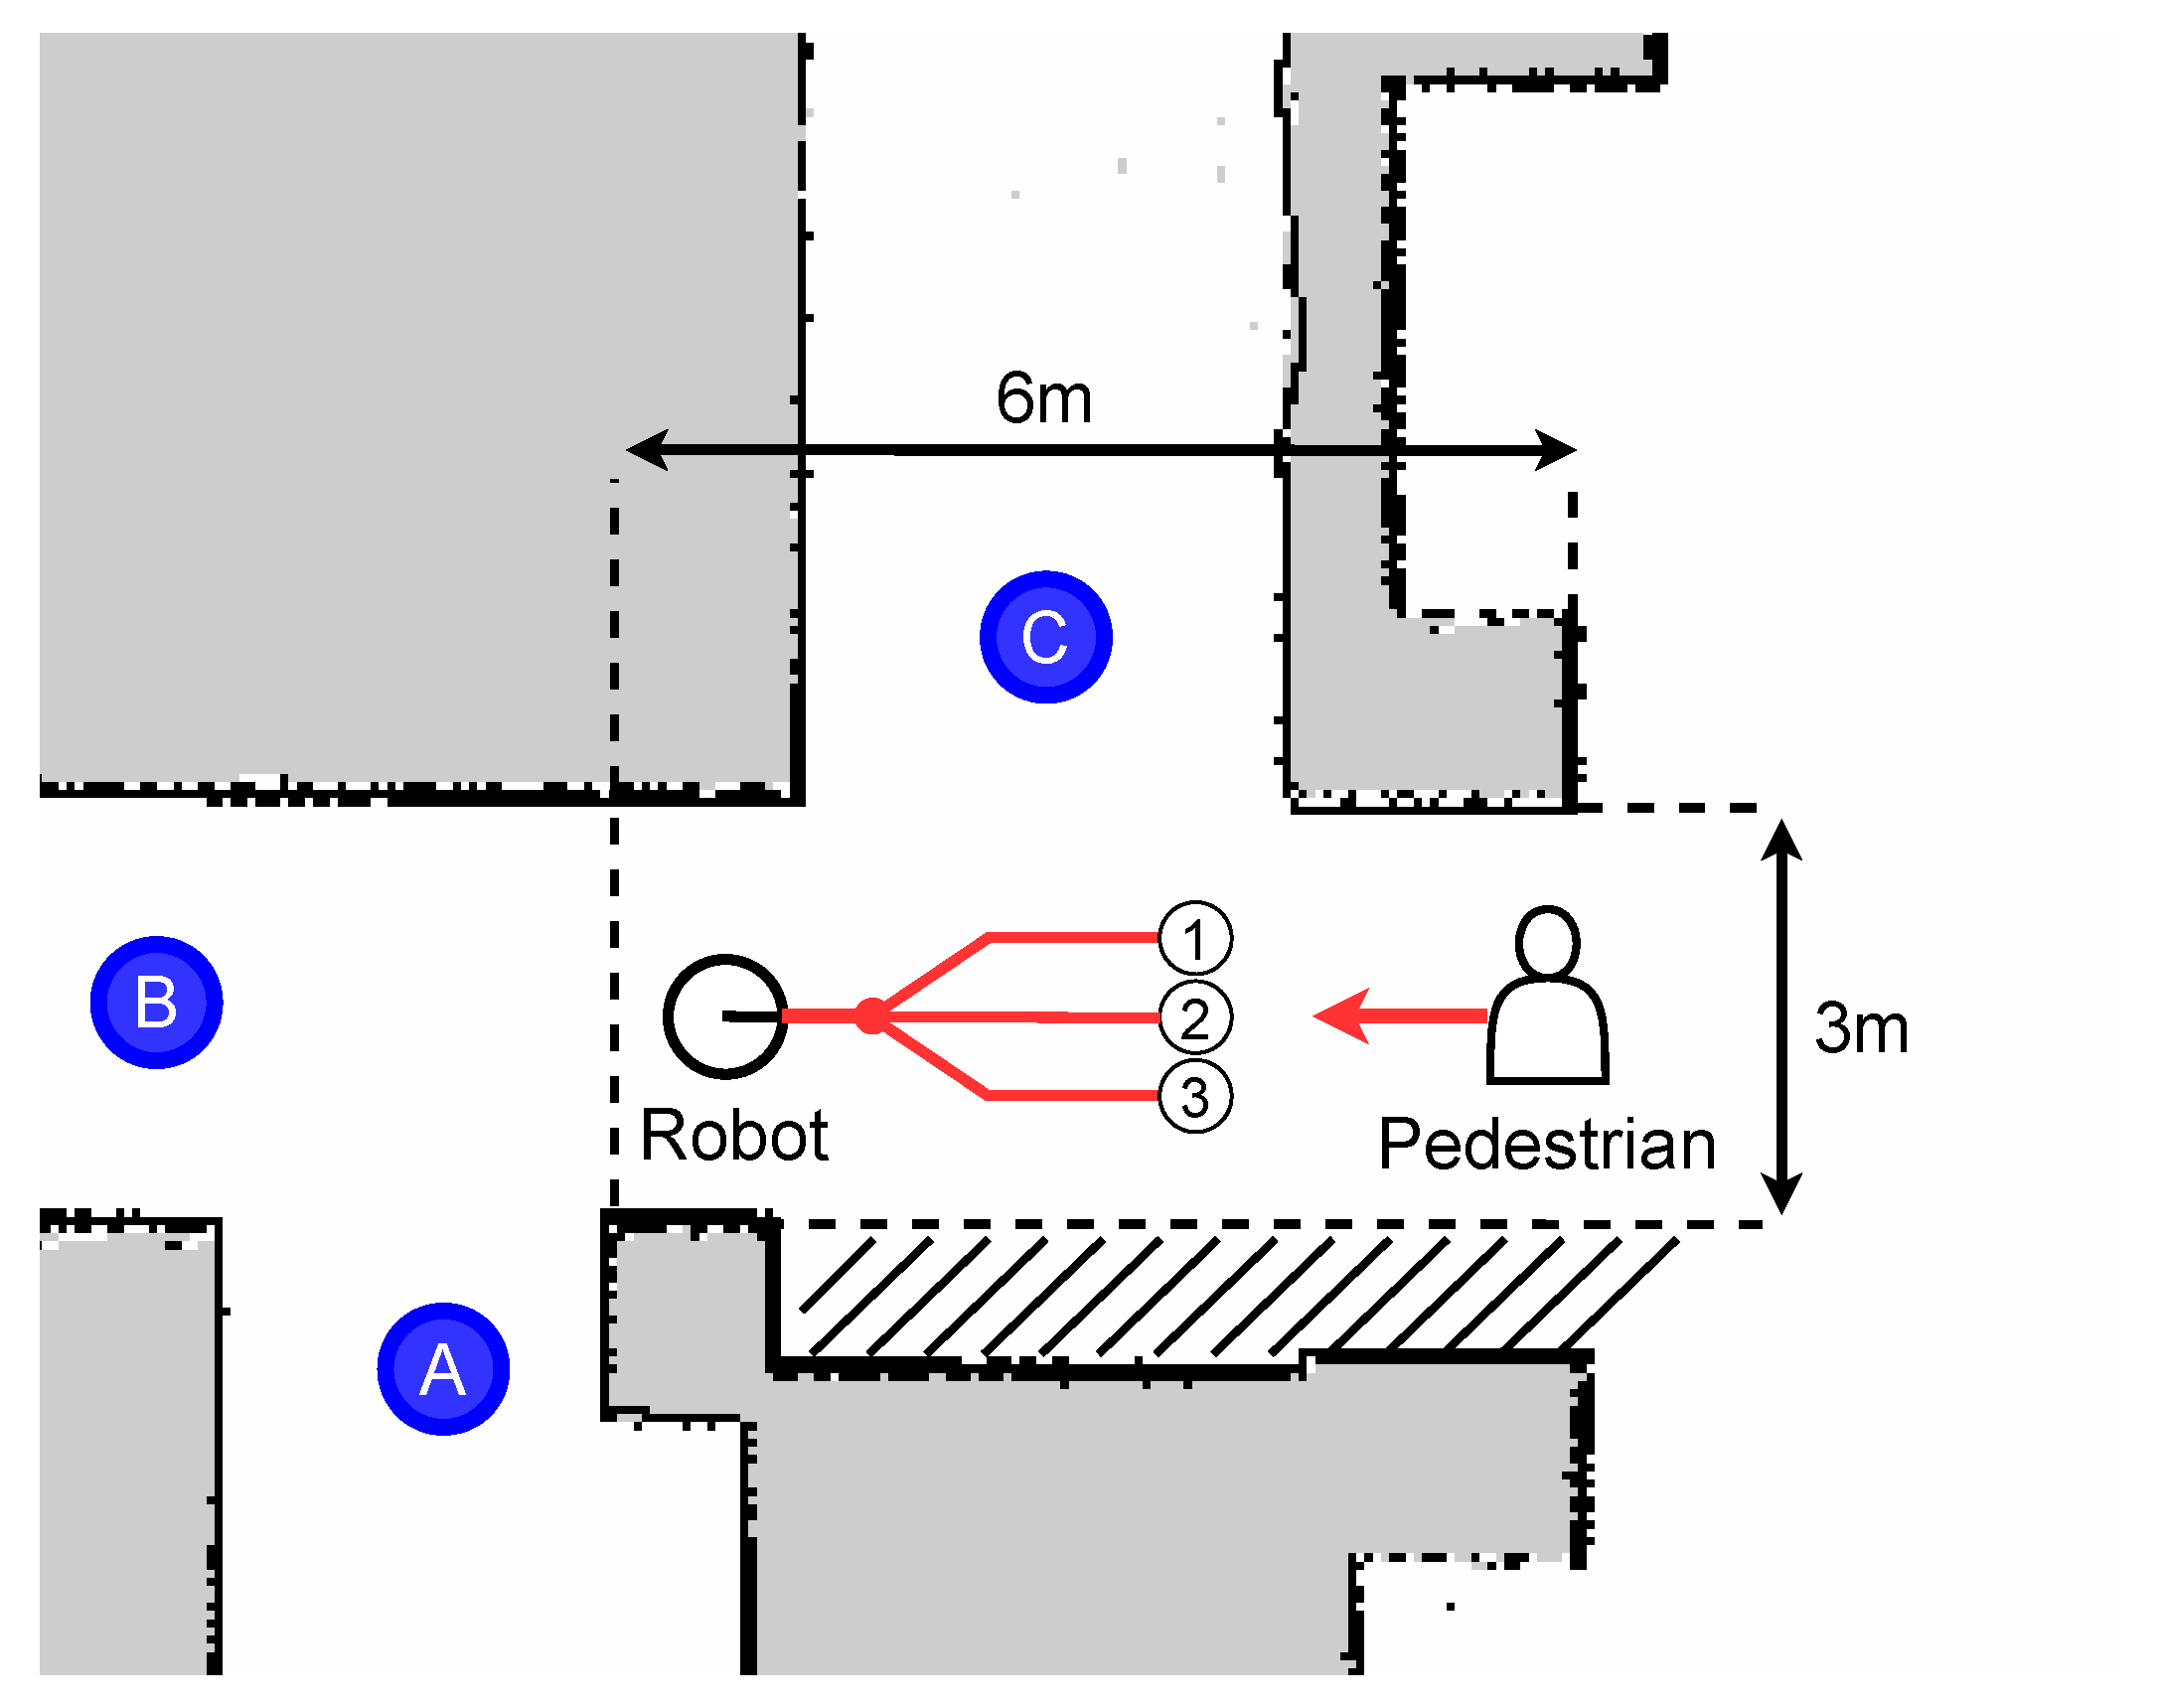
\includegraphics[keepaspectratio, scale=0.27]
      {images/oculus_experiments.pdf}
\caption{Experimental environment}
 \label{Fig:oculus-exp-overview}
\end{figure} 

\begin{figure}[H]
  \centering
  \begin{minipage}{0.42\textwidth}
    \centering
    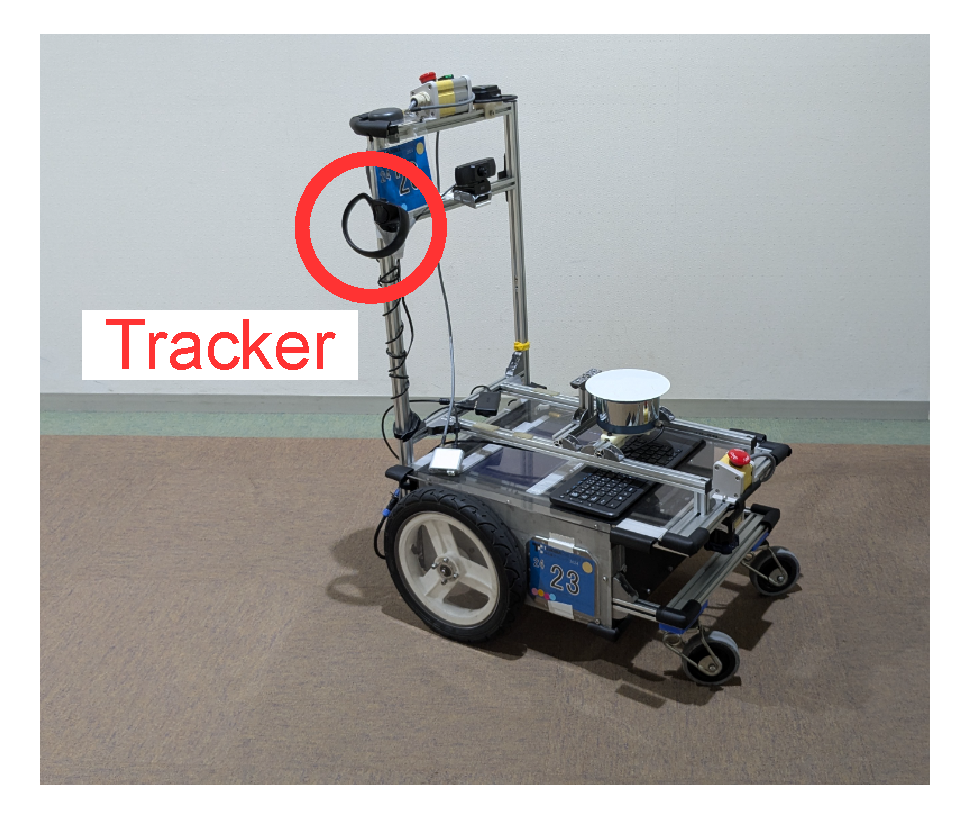
\includegraphics[width=\textwidth]{images/tracking-robot.pdf}
    \subcaption{Robot}
    \label{fig:tracking-robot}
  \end{minipage}
  % \hfill
  \begin{minipage}{0.42\textwidth}
    \centering
    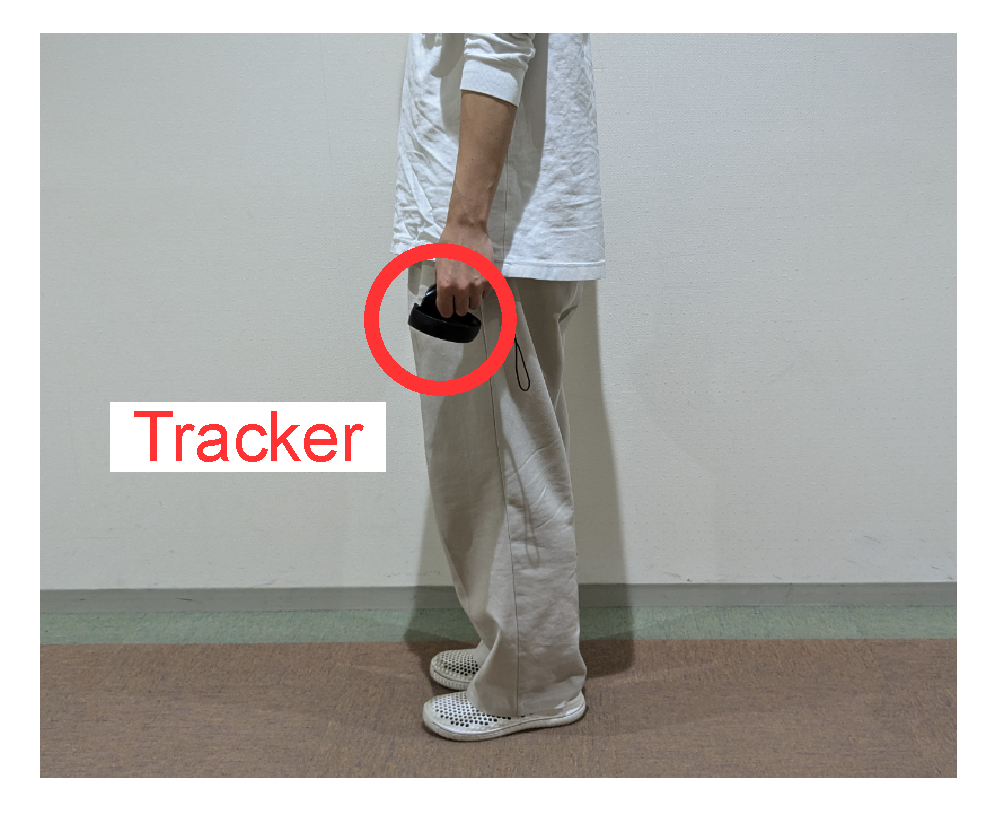
\includegraphics[width=\textwidth]{images/tracking-ped.pdf}
    \subcaption{Pedestrian}
    \label{fig:tracking-ped}
  \end{minipage}
  \caption{Tracking sensor setup}
  \label{fig:tracking}
\end{figure}

\vspace{-20pt}

\begin{figure}[H]
  \centering
 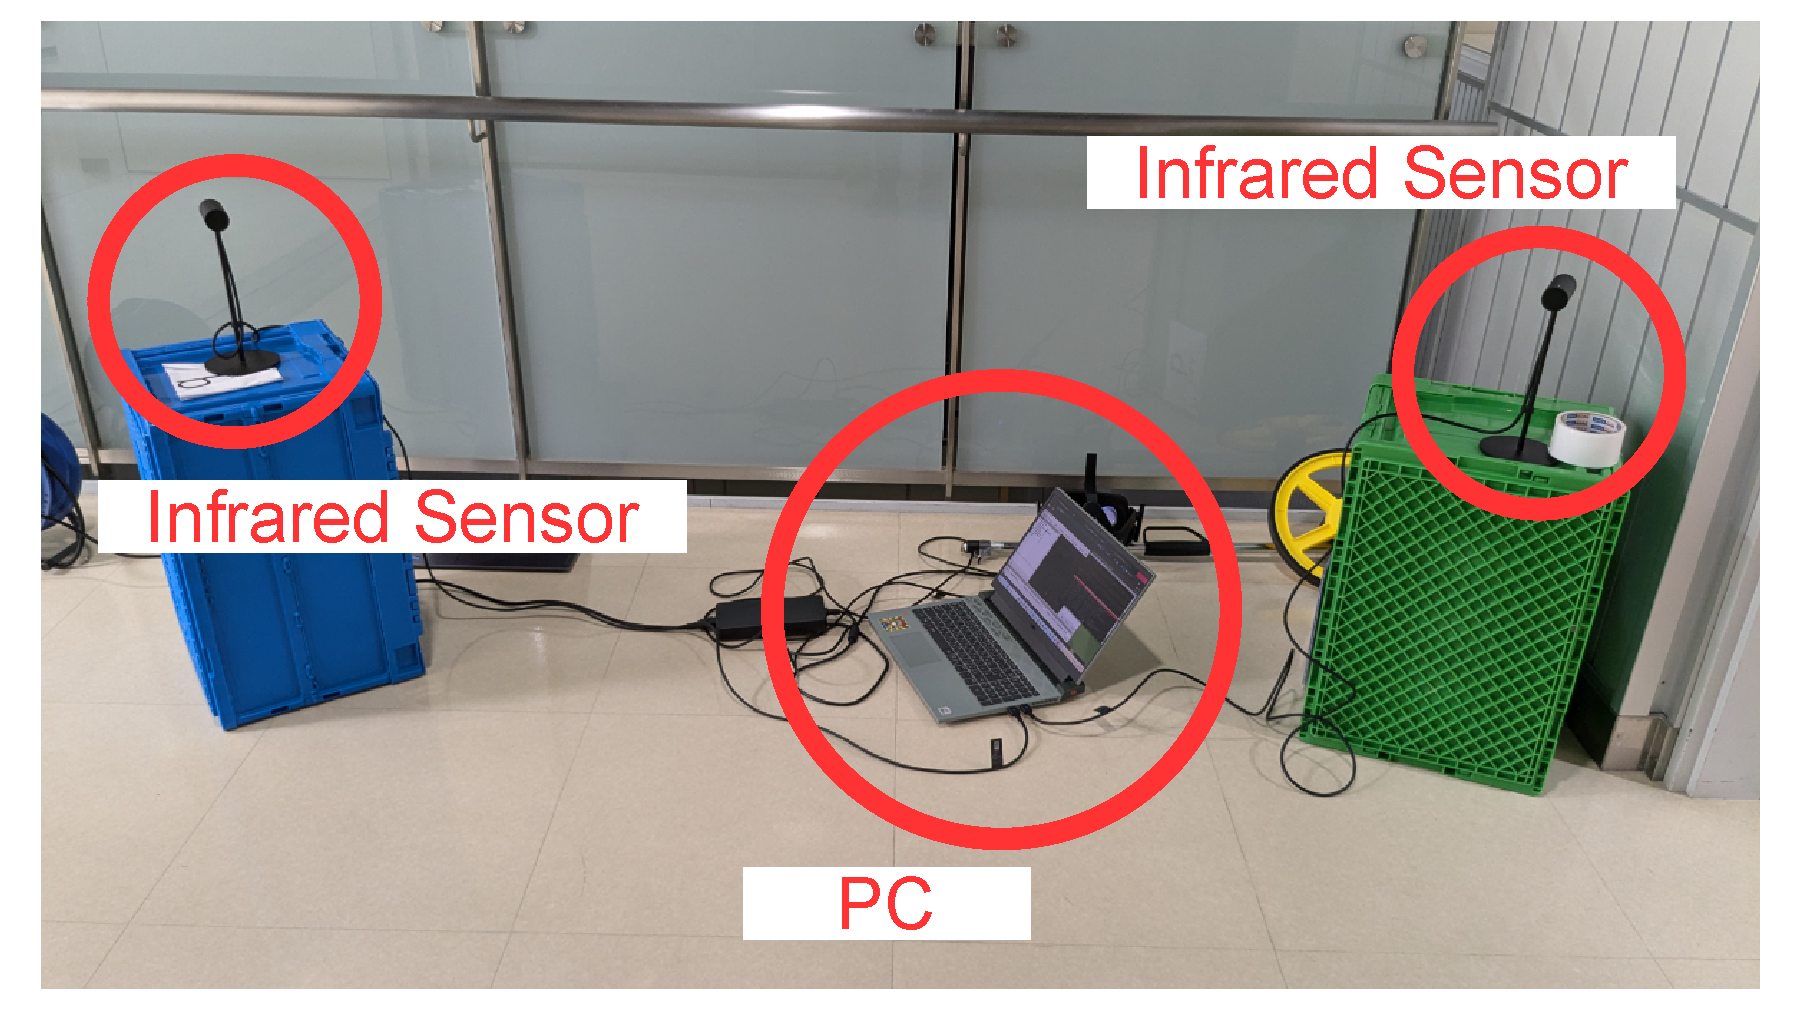
\includegraphics[keepaspectratio, scale=0.32]
      {images/tracking-sensor.pdf}
\caption{Infrared sensor setup}
 \label{Fig:oculus-sensor}
\end{figure}

\vspace{-20pt}

\section{結果と考察}\label{sec:oculus-exp-result}
\tabref{tab:robot-behavior}に,ロボットの行動を考慮する場合と考慮しない場合における各評価指標の値を示す.ロボットの行動を考慮しない場合と比較して,ADEは7.5%,FDEは15.9%誤差低減が確認できる.
この結果から,ロボットの行動を考慮することで,歩行者の軌道予測の精度が向上することが分かる.特にFDEの改善が顕著であり,ロボットの動きが歩行者の最終的な位置に大きな影響を与えていることを示唆している可能性がある.一方で,ADEの改善幅は比較的小さく,\figref{Fig:oculus-exp-overview}に示したように,3箇所の目的地のうち2箇所で角を曲がる必要があるため,途中の軌道予測が困難になり,評価指標の値の向上幅が抑えられたと考えられる.

\begin{table}[H]
  \begin{center}
  \caption{Comparison with and without taking into account the robot's behavior}
  \label{tab:robot-behavior}
  % \footnotesize
  \begin{tabular}{c||c|c}
   & ADE & FDE \\ 
  \hline \hline
  Normal      & 0.40       & 0.69                      \\
  \hline
  Considering robot behavior    & 0.37       & 0.58                      \\
  \hline
  \end{tabular}
  \end{center}
\end{table}

\figref{Fig:pred-straight},\figref{Fig:pred-right},\figref{Fig:pred-left}は,実験で取得した目的地Aへの歩行データに対する予測例である.これらの例では,ロボットが行動を取り始める時刻を最終観測時刻とした.ロボットの行動を考慮しない場合は,いずれのロボット挙動に対しても回避行動を伴う予測が見られなかった.
一方,ロボットの行動を考慮した予測では,より真値に近い軌道を推定している様子が確認できる.
観測時間内においては,歩行者の行動は一貫して直進していたため,その後のロボットを回避する動きを予測することは本来困難である.しかし,\figref{Fig:pred-straight},\figref{Fig:pred-right}ではロボットを回避するような予測が確認できる.このことから,ロボットの行動を考慮する軌道予測が歩行者とロボット間の相互作用を適切に捉えていると考えられる.

\vspace{-10pt}

\begin{figure}[H]
  \centering
 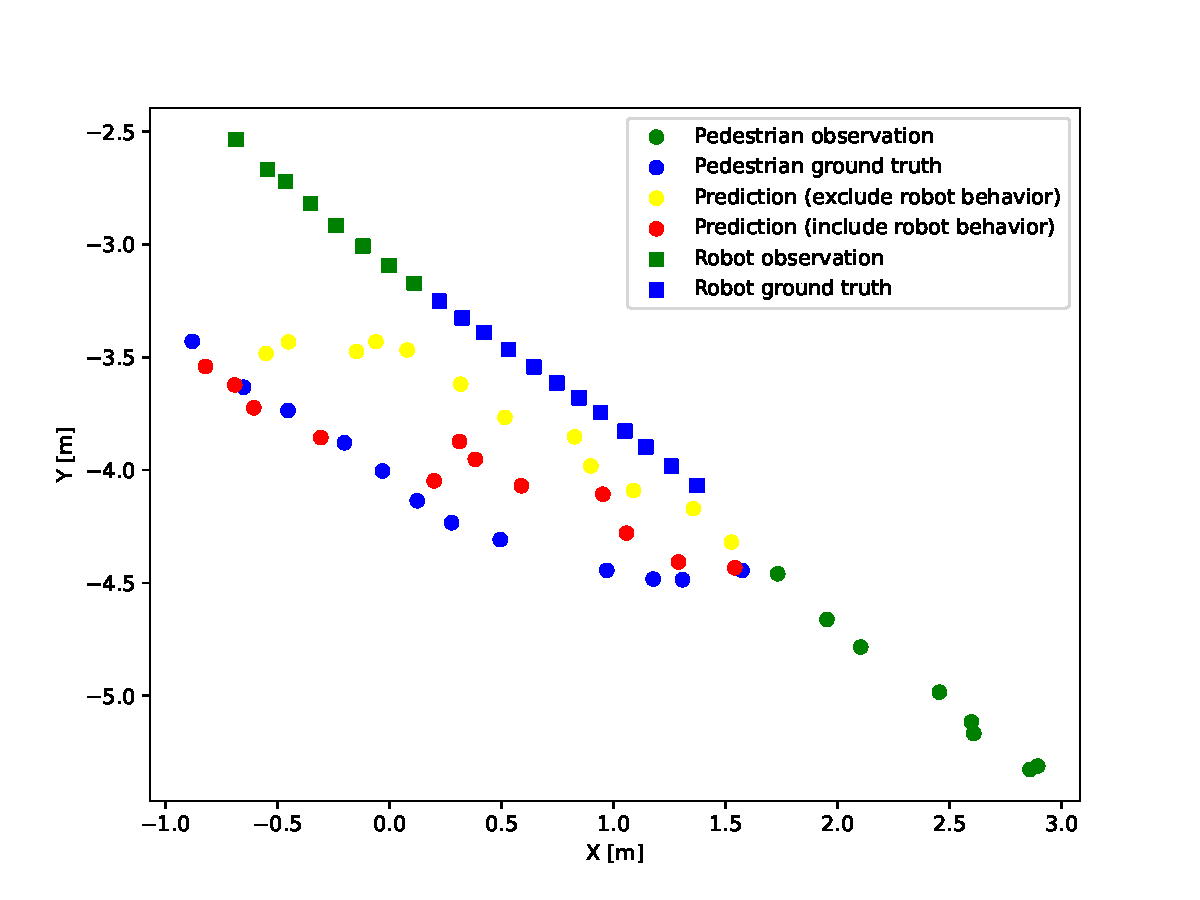
\includegraphics[keepaspectratio, scale=0.58]
      {images/pred_straight.pdf}
\caption{Predicted trajectory when the robot moves straight}
 \label{Fig:pred-straight}
\end{figure}

\begin{figure}[H]
  \centering
 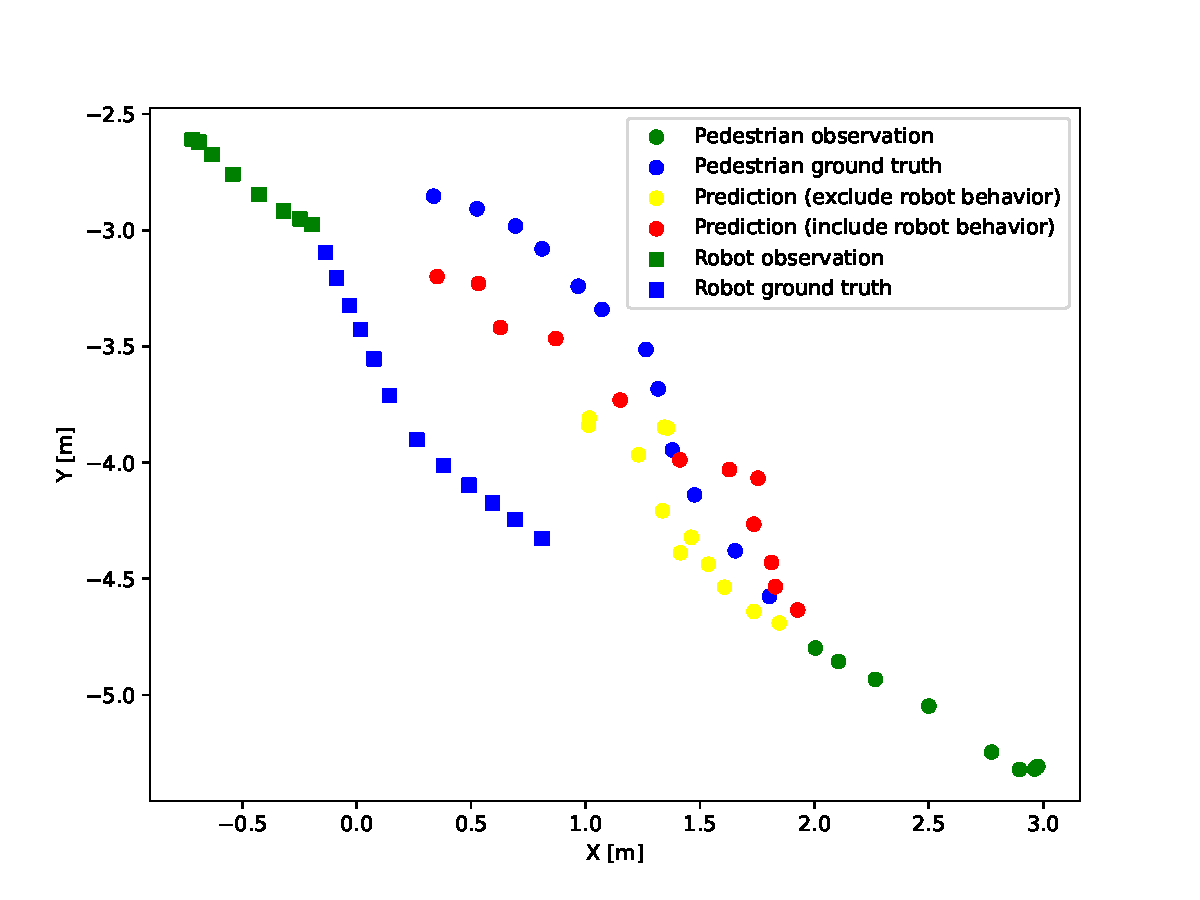
\includegraphics[keepaspectratio, scale=0.58]
      {images/pred_right.pdf}
\caption{Predicted trajectory when the robot moves right}
 \label{Fig:pred-right}
\end{figure}

\vspace{-30pt}

\begin{figure}[H]
  \centering
 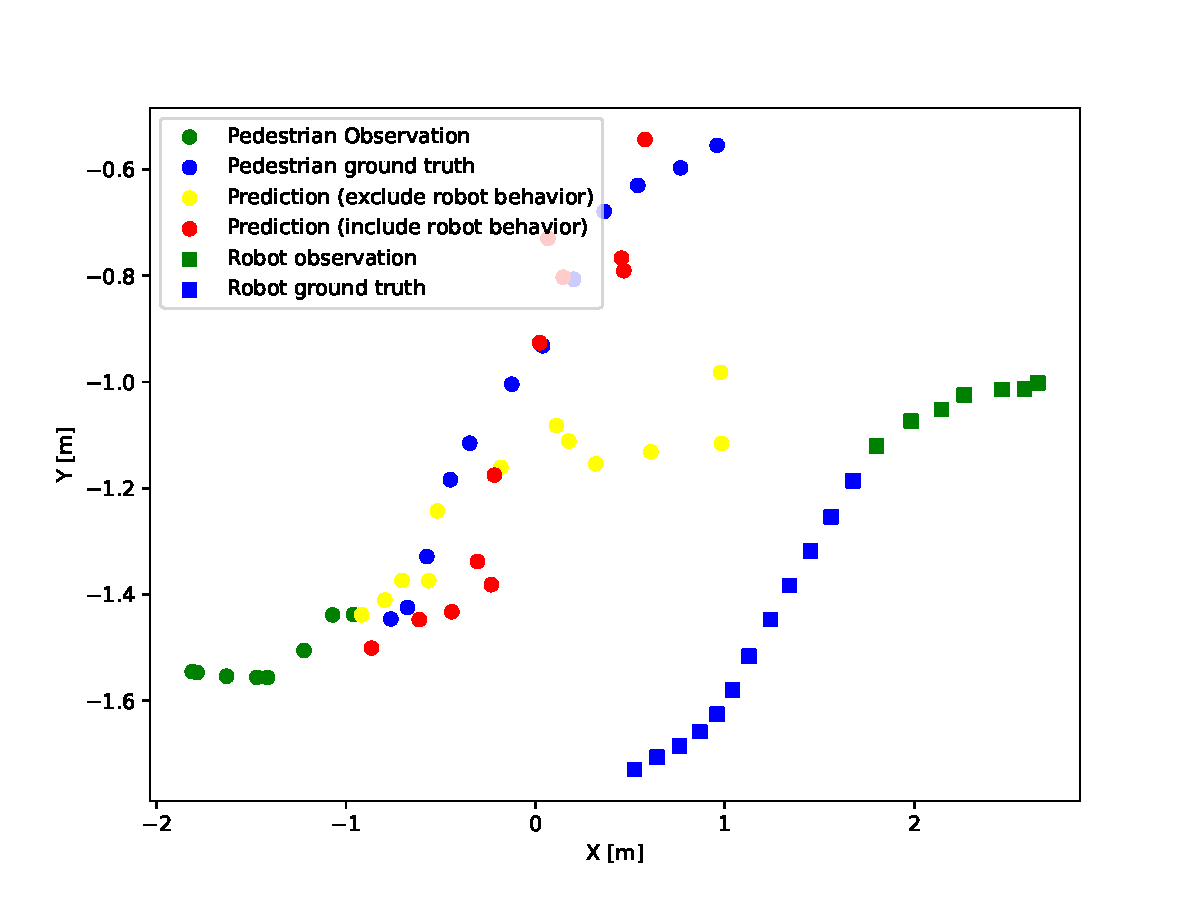
\includegraphics[keepaspectratio, scale=0.58]
      {images/pred_left.pdf}
\caption{Predicted trajectory when the robot moves left}
 \label{Fig:pred-left}
\end{figure}

\newpage
